%% ============================================================================
%%  Sponsor Exposure Analytics for the Rest of Us: An Open, Self-Hostable
%%  Framework for Small and Mid-Tier Sports Clubs
%%
%%  Target venue : TBD (IEEE CyberWorlds / ACM MMSports workshop / CVsports
%%                 workshop — decide with advisor, see paper_outline_for_advisor.md)
%%  Format       : IEEEtran conference, 2-column. Compile on Overleaf or:
%%                   latexmk -pdf main_accessibility.tex
%%
%%  NOTE ON NUMBERS: remaining \TODOnum{...} (red) are PLACEHOLDERS. Detection
%%  numbers are now real, verified against logo_detection/runs/*/results.csv:
%%    - random-frame split   : logo_yolo26m        best mAP@0.5 = 0.862
%%    - clip-disjoint split  : logo_yolo26m_clipsplit  best mAP@0.5 = 0.702
%%    - extended data (v2)   : logo_yolo26m_v2_full-2  best mAP@0.5 = 0.745 (P .65 R .74)
%%  CONFIRM before submission: the 0.862 run predates the clip-split fix (split
%%  provenance inferred from run names — all args.yaml point at the same
%%  data.yaml path, regenerated in place). RF-DETR run (training-result/,
%%  ema mAP@0.5 = 0.778) used Roboflow's RANDOM split -> not citable as-is.
%%  Do NOT submit while any \TODOnum remains.
%%  NOTE ON CLUB IDENTITY: the deploying club's name is intentionally withheld
%%  throughout for client confidentiality — keep it that way in any edits.
%%  FIGURE POLICY (user decisions 2026-07-10/11): sponsor logo crops may be
%%  shown un-redacted (Fig. 3); the club NAME, crest, scoreboards, and club-TV
%%  watermarks must never appear in a figure. Fig. 4 timeline keeps sponsors
%%  anonymized/numbered (text lists names more directly than a small crop).
%% ============================================================================
\documentclass[conference]{IEEEtran}
\IEEEoverridecommandlockouts

\usepackage{cite}
\usepackage{amsmath,amssymb,amsfonts}
\usepackage{graphicx}
\usepackage{booktabs}
\usepackage{xcolor}
\usepackage{url}
\usepackage[colorlinks=true,allcolors=blue]{hyperref}
\usepackage{tikz}
\usepackage{pgfplots}
\pgfplotsset{compat=1.18}
\usetikzlibrary{positioning,arrows.meta,shapes.geometric,fit,backgrounds,calc}

% --- placeholder helper: makes unfilled numbers visually obvious -------------
\newcommand{\TODOnum}[1]{{\color{red}\textbf{#1}}}

% --- shared tikz styles (kept consistent with the companion CyberWorlds draft) -
\tikzset{
  blk/.style   ={rectangle, rounded corners=2pt, draw=black!70, thick,
                 fill=blue!6, align=center, inner sep=4pt, font=\scriptsize,
                 minimum height=8mm, text width=22mm},
  data/.style  ={rectangle, draw=black!55, fill=gray!8, align=center,
                 inner sep=3pt, font=\scriptsize\itshape, text width=20mm},
  teach/.style ={blk, fill=orange!12},
  stud/.style  ={blk, fill=green!12},
  arr/.style   ={-{Stealth[length=2mm]}, thick, draw=black!65},
}

\begin{document}

\title{Sponsor Exposure Analytics for the Rest of Us: An Open, Self-Hostable\\
Framework for Small and Mid-Tier Sports Clubs}

\author{\IEEEauthorblockN{First Author\IEEEauthorrefmark{1},
Second Author\IEEEauthorrefmark{1}}
\IEEEauthorblockA{\IEEEauthorrefmark{1}Affiliation\\
\texttt{\{author1,author2\}@inst.edu}}}

\maketitle

% ============================================================================
\begin{abstract}
Measuring how long and how prominently a sponsor's logo appears in match video, and
converting that exposure into an estimated media value (EMV), is a well-served problem
for clubs that can afford an enterprise vendor (Nielsen Sports, GumGum/Zoomph, Relo
Metrics, Shikenso) or that maintain an in-house data-science team — and, in practice,
for clubs whose matches are covered by an official broadcast feed those vendors can
integrate with in the first place. Most professional clubs outside the top-revenue
leagues have neither the budget nor a broadcast deal. We present an end-to-end,
self-hosted framework that a club can use to ingest \emph{its own} match video —
whatever it is able to capture itself, not necessarily an official broadcast feed — and
turn it into sponsor exposure and media-value reports. The framework is assembled
entirely from open-source models and libraries, deployable on commodity hardware, and
deployed and evaluated at a real professional sports club whose identity we withhold for
confidentiality. Beyond detection, the framework resolves two problems that prior
published systems leave open: attributing each detected logo to the correct team when
the same sponsor appears on both sides' kits, advertising boards, or officials; and
pricing sponsor placements at the level of individual kit slots rather than only
aggregate screen time. We position our pricing formula explicitly against existing
valuation practice — both the manual Advertising/Earned Media Value Equivalency (AVE)
methodology used across the sponsorship industry, and recent AI-driven valuation
systems — and show that neither line of work prices exposure below the level of a
brand's total on-screen time. On self-ingested match video from a real fixture, the
framework tracks players, filters out opponent-owned instances of shared sponsors, and
produces
per-brand and per-placement exposure and EMV reports; we report detection accuracy on a
clip-disjoint split (mAP@0.5 = 0.75; the same detector evaluated under a naive
random-frame split reaches 0.86, a gap we report explicitly as evidence of
split-induced inflation rather than model quality), team-attribution behaviour on an
initial set of labelled clips, and the scale of the overcounting that attribution
prevents: across eight of nine full-match deployment videos, 41\% of raw logo
detections belonged to opponents or officials, or were unattached to any tracked
player, and would otherwise have been priced as the target club's kit exposure; the
ninth match, flagged by a visual audit, is reported as a failure case of the team
classifier rather than as filtering. We report the design choices, calibration lessons, and
failure modes needed to take a sponsor-analytics system from paper to a low-cost,
production deployment.
\end{abstract}

\begin{IEEEkeywords}
sponsor visibility, media value equivalency, logo detection, team attribution, sports
analytics, open-source, accessibility, self-service video ingestion.
\end{IEEEkeywords}

% ============================================================================
\section{Introduction}
\label{sec:intro}

Sports clubs sell advertising space on their kits, but only a small number of clubs can
verify what that space is actually worth. Our partner club — a professional club that
sells sponsor slots on its kit but, like most clubs outside the top handful of leagues,
has no in-house analytics team and no enterprise sponsorship-measurement contract — is
representative of the majority of the market this paper targets. (We withhold the
club's name throughout this paper for commercial confidentiality; nothing in the
results depends on the club's identity.)

A commercial layer already serves the sponsor-measurement need: Nielsen's sponsorship
benchmarking~\cite{nielsen_sponsorship_benchmark}, GumGum/Zoomph, Relo
Metrics~\cite{relometrics_ai}, and Shikenso all offer automated or semi-automated
sponsor-visibility services. These are delivered as closed, hosted platforms: a club
sends its footage to a third party and receives a report back, typically under a
recurring contract, typically by integrating with an official broadcast feed. This is a
reasonable model for a club with the budget, the appetite for such a contract, and a
broadcast deal to plug into — but it leaves three structural costs unaddressed for
everyone else: vendor lock-in and recurring fees; the requirement to hand a club's raw
video and commercial sponsorship data to an external party rather than keeping it
in-house; and, for the many clubs with no official broadcast coverage at all, a
dependency on broadcast access that simply does not exist for them regardless of
budget. Our framework instead is built around \emph{self-service ingestion}: a club
uploads whatever match video it is able to capture itself — a fixed pitch-side camera,
a livestream recording, footage from a coach's or media officer's own filming — and the
system produces exposure and EMV reports from that, with no dependency on an official
broadcast feed or a vendor integration. We target clubs for whom these costs — not
detection accuracy — are the binding constraint. To be precise about what we mean by ``accessible'': self-hosting
removes cost and vendor lock-in, but it does not remove the need for some technical
capacity to operate the system; our claim is narrower than ``any club, zero technical
skill'' and is better stated as ``clubs with modest technical capacity but no
analytics budget or vendor contract.''

Even with a working, open-source logo detector, two problems remain unresolved by the
closest published system, ExposureEngine~\cite{exposureengine} (\S\ref{sec:related}).
First, the same sponsor frequently appears on both competing teams' kits, on
perimeter advertising boards, or on match officials, so raw detection systematically
overcounts a sponsor's exposure unless ownership is resolved per detected instance.
Second, sponsors are priced by placement in practice — a chest-centre logo is worth
more than one on a sock — yet no published system we are aware of attributes exposure,
or price, at that granularity.

\noindent\textbf{Contributions.}
\begin{itemize}
  \item \textbf{C1.} A formulation and training-free solution for
  \emph{team attribution}: resolving which team owns a detected logo instance without
  training a separate model per opponent, using a reference-based bootstrap, appearance
  fusion, and track-level temporal voting.
  \item \textbf{C2.} A three-tier, zero-manual-setup reference bootstrap for team
  attribution (manual override $\to$ kit-anchor auto-clustering $\to$ luminance
  heuristic), so the system requires no per-match human configuration.
  \item \textbf{C3.} \emph{Placement-level pricing}: attributing exposure, and
  therefore price, to eighteen individual kit slots via pose estimation — a granularity
  absent from both the manual AVE/EMV literature and recent AI-driven valuation systems
  (\S\ref{sec:related}).
  \item \textbf{C4.} An open reference architecture assembled entirely from
  open-source models and libraries, built around \emph{self-service video ingestion}
  rather than a broadcast-feed integration, with infrastructure abstracted behind
  swappable interfaces so that a club can start at near-zero infrastructure cost, with
  no dependency on having a broadcast deal, and scale only if and when needed.
  \item \textbf{C5.} Production-grade design and calibration lessons from a real
  deployment: a two-pass sampled/full-fps detection trade-off, graceful degradation
  under partial failure, and two specific calibration corrections (visibility threshold,
  train/test leakage) that changed our reported numbers substantially.
\end{itemize}
Of these, C1 and C3 are the primary technical claims; C2, C4, and C5 are supporting
system contributions that make C1 and C3 practical to deploy.

% ============================================================================
\section{Related Work}
\label{sec:related}

\subsection{Logo detection}
Logo detection is a comparatively mature problem~\cite{logo_detection_survey}; we build
on a standard fine-tuned open-weight detector rather than proposing a new detection
architecture, and treat detection accuracy as a means to an end rather than as this
paper's contribution.

\subsection{Team classification and jersey-based re-identification}
Assigning a detected player to a team from jersey appearance is an active area in its
own right, including joint re-identification, team-affiliation, and role classification
for sports tracking~\cite{team_reid_roles}, jersey-number recognition under
uncertainty~\cite{jersey_number_cvsports}, and earlier work combining spatial
constellation features with jersey-number recognition for player
identification~\cite{soccer_player_recognition}; see also the broader computer-vision-
in-sports survey~\cite{cv_sports_survey}. Most of this literature performs per-frame
colour or embedding clustering for team assignment. We build directly on this and add a
track-level temporal voting scheme with hysteresis, together with a zero-manual-setup
reference bootstrap — the differentiation is in \emph{how} team identity is made
stable and cheap to configure per match, not in team classification itself.

\subsection{Ad-board localization in broadcast video}
A separate, older line of work localizes static advertising surfaces in broadcast video
in order to insert or replace advertising content: implanting virtual advertisements
into broadcast soccer video~\cite{virtual_ad_insertion}, automated billboard
insertion~\cite{billboard_insertion}, and billboard-advertisement
detection~\cite{billboard_detection_sport_tv}. This literature solves a related but
different problem — inserting or replacing an ad on a located surface — whereas we
measure the exposure of sponsors that are already, physically, on screen.

\subsection{Automated sponsor-visibility systems}
The closest published system is ExposureEngine~\cite{exposureengine}, which introduces
an oriented-bounding-box detector for sponsor logos and a visibility/exposure analytics
pipeline for soccer broadcasts, reporting mAP@0.5 of 0.859 on a purpose-built Swedish
top-flight soccer dataset drawn from official broadcast coverage. As far as its
published description shows, it does not address logos shared between opposing teams
or officials, does not attribute exposure below brand level, does not discuss
deployment cost, and — like the commercial vendors below — assumes access to an
official broadcast feed rather than club-captured video. This last point matters in
practice: most clubs outside the top leagues have no broadcast coverage to draw on at
all, independent of budget. Commercial vendors
(Nielsen~\cite{nielsen_sponsorship_benchmark}, GumGum/Zoomph, Relo
Metrics~\cite{relometrics_ai}, Shikenso) confirm that the underlying problem is
commercially important, but their methods are closed, unpublished, and not independently
reproducible.

\subsection{Existing pricing and valuation models — manual and AI-driven}
\label{sec:related-pricing}
The industry-standard manual approach is Advertising/Earned Media Value Equivalency
(AVE/EMV): convert the size, duration, and placement of exposure into the cost of an
equivalent slot of paid advertising, typically via a hand-set placement multiplier. Our
own Tier-3 pricing formula (\S\ref{sec:emv}) is drawn from exactly this family of
formulas, as used in prior industry and academic practice, and we cite it directly here
rather than treating it as generic background. The AVE methodology is also the target of
sustained, public criticism from industry bodies — AMEC, IPR, PRSA, PRCA, and ICCO have
each issued position statements rejecting AVE as unreliable~\cite{ave_criticism},
citing arbitrary multipliers, no signal for content or audience sentiment, and treating
every viewer as identical regardless of placement or audience quality. Our
placement-level pricing (C3) makes one specific weakness of this criticism — the
arbitrariness of a single, flat multiplier — more principled, by grounding a portion of
the multiplier in measured, per-slot exposure share; it does \emph{not} address the
deeper criticism that AVE-style metrics ignore audience quality, sentiment, or brand
recall, and we state this as an explicit scope limitation
(\S\ref{sec:discussion}) rather than imply the pricing problem is solved.

On the AI-driven side, recent systems apply machine learning directly to sponsorship
valuation: SSPAIN.ai~\cite{sspain_ai}, a survival-analysis model trained on more than
5{,}800 historical sponsorships to forecast sponsorship renewal probability and
duration, and Relo Metrics'~\cite{relometrics_ai} combined
computer-vision-and-machine-learning pipeline for automated media value and dynamic
pricing. Both are methodologically related to more general machine-learning-based
dynamic pricing, e.g.\ in e-commerce~\cite{dynamic_pricing_ml_ecommerce}, which reacts
to real-time demand signals rather than sports-specific placement data. None of this
AI-driven work, as far as published material shows, prices exposure below the level of
a brand's aggregate on-screen time, and none discusses low-cost or self-hosted
deployment.

\subsection{Summary of the gap}
No published work we are aware of simultaneously addresses (a) team/opponent-overlap
attribution, (b) placement-level pricing, in either the manual or AI-driven valuation
literature, and (c) deployment accessibility for clubs without an enterprise budget or
an in-house ML team. This is the gap this paper targets.

% ============================================================================
\section{System Architecture}
\label{sec:arch}

\begin{figure*}[t]
\centering
% Fig. 1 — End-to-end pipeline (orchestrated stages, graceful degradation)
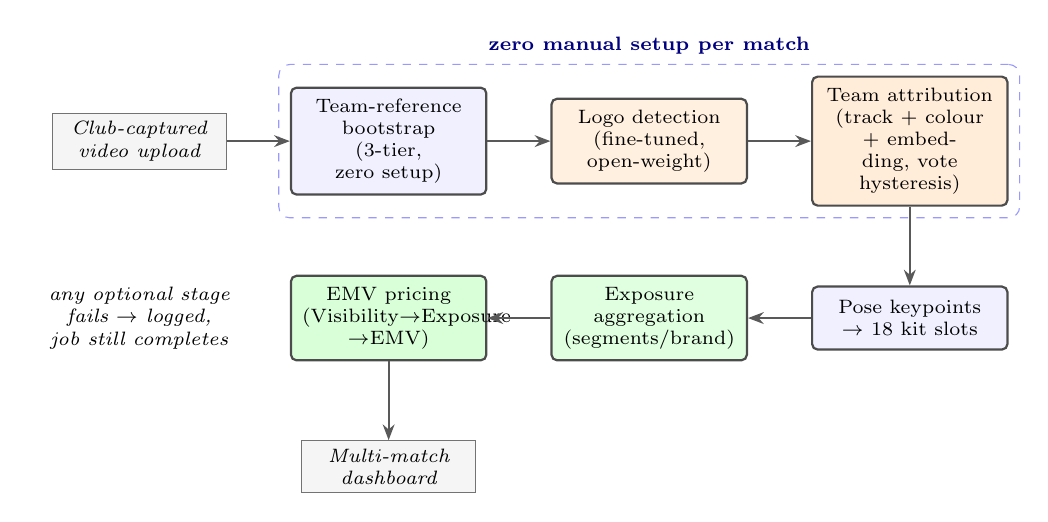
\begin{tikzpicture}[node distance=6mm and 8mm]
  % input
  \node[data] (video) {Club-captured\\video upload};

  % bootstrap + detect
  \node[blk, right=of video] (bootstrap) {Team-reference\\bootstrap\\(3-tier, zero setup)};
  \node[teach, right=of bootstrap] (detect) {Logo detection\\(fine-tuned,\\open-weight)};

  % team attribution
  \node[blk, right=of detect, fill=orange!15, text width=22mm]
       (team) {Team attribution\\(track + colour\\+ embedding, vote\\hysteresis)};

  % pose / body zone
  \node[blk, below=10mm of team, text width=22mm] (pose) {Pose keypoints\\$\to$ 18 kit slots};

  % exposure + pricing
  \node[stud, left=of pose] (exposure) {Exposure\\aggregation\\(segments/brand)};
  \node[stud, left=of exposure, fill=green!15] (pricing) {EMV pricing\\(Visibility$\to$Exposure\\$\to$EMV)};

  % output
  \node[data, below=10mm of pricing] (dash) {Multi-match\\dashboard};

  % grouping box for the parts a club never has to touch manually
  \begin{scope}[on background layer]
    \node[draw=blue!40, dashed, rounded corners, fit=(bootstrap)(detect)(team),
          inner sep=4pt,
          label={[font=\scriptsize\bfseries,blue!50!black]above:zero manual setup per match}] {};
  \end{scope}

  % arrows
  \draw[arr] (video) -- (bootstrap);
  \draw[arr] (bootstrap) -- (detect);
  \draw[arr] (detect) -- (team);
  \draw[arr] (team) -- (pose);
  \draw[arr] (pose) -- (exposure);
  \draw[arr] (exposure) -- (pricing);
  \draw[arr] (pricing) -- (dash);

  % graceful degradation note — sits in the empty left column of the second row
  \node[font=\scriptsize\itshape, text width=26mm, align=center]
       at (video |- pricing) {any optional stage fails $\to$ logged, job still completes};
\end{tikzpicture}

\caption{\textbf{End-to-end pipeline.} An orchestrated job runs frame sampling, a
zero-manual-setup team-reference bootstrap, logo detection, team attribution, pose-based
kit-slot assignment, exposure aggregation, and EMV pricing, feeding a multi-match
dashboard. Every optional stage degrades gracefully on failure rather than aborting the
job, and infrastructure (storage, database, job queue) sits behind swappable interfaces
so a deployment can start at near-zero cost.}
\label{fig:pipeline}
\end{figure*}

The system is organized as a single orchestrated job per uploaded video
(Fig.~\ref{fig:pipeline}). Two design choices are central to the accessibility claim.
First, every optional pipeline stage degrades gracefully: if a stage's dependency is
unavailable (e.g.\ no team reference could be bootstrapped), the stage is skipped and
logged rather than failing the job, so a club always gets a usable, if partial, result.
Second, infrastructure is abstracted behind swappable interfaces: the default
configuration uses local file storage, an embedded database, and an in-process job
queue, with an optional, opt-in path to object storage, a managed database, and a
distributed queue for clubs whose volume justifies it. A deployment therefore starts at
near-zero infrastructure cost and only incurs additional cost when actually needed.

The pipeline also separates two passes over the video at different sampling rates: a
sparsely sampled pass drives the exposure/EMV numbers (accurate enough for aggregate
timing at a fraction of the compute cost), and a full-frame-rate pass produces a smooth
annotated preview for human review. This trade-off is explicit and reported
(\S\ref{sec:exp}) rather than hidden inside a single, uniformly-sampled detection pass.

% ============================================================================
\section{Method}
\label{sec:method}

\subsection{Detection and annotation}
The logo detector is a YOLO26m model fine-tuned at 1280-pixel input on manually
annotated frames drawn
from the same kind of video the framework is meant to run on in deployment — video a
club captures and uploads itself, not necessarily an official broadcast feed, and
therefore potentially more variable in camera stability, framing, and production
quality than the broadcast-sourced footage used to train and evaluate prior published
detectors. To reduce annotation cost, we use a model-assisted labelling loop: a small
hand-labelled seed set (on the order of tens of images per class) trains an early model,
which then proposes boxes on new frames for a human to accept, correct, or reject,
before a final model is trained on the combined set. This does not eliminate manual
annotation, and we treat the remaining annotation cost explicitly as the main residual
barrier to full accessibility (\S\ref{sec:future}), rather than claiming an
annotation-free pipeline in this paper. Per-frame detection sits behind a swappable
backend interface, so a transformer-based detector (RF-DETR) can replace the YOLO
backend without touching the rest of the pipeline; all detection numbers reported in
this paper use the YOLO26m backend. In deployment, detections below a confidence
floor of 0.25 are discarded, but confidence is otherwise used as a continuous weight
in the visibility score (\S\ref{sec:emv}) rather than as a gate — a deliberately
recall-first choice: in our deployment data, detections with confidence below 0.4
account for 29\% of pose-attributed detections but only 9.5\% of quality-weighted
exposure, so genuine small or motion-blurred kit logos are retained at little cost to
the aggregate, and spurious ones are further suppressed by the minimum-duration rule
of \S\ref{sec:emv}.

\subsection{Team attribution}
\label{sec:teamfilter}
Detected persons are tracked across frames; for each track, a jersey crop is classified
by fusing a colour histogram with a general-purpose vision embedding, and
classifications are accumulated per track with hysteresis, so that a single blurred or
occluded frame cannot flip an already-confident team label. Reference examples for each
kit are obtained automatically rather than by manual setup: from official kit images
when available, and otherwise by clustering the video's own early frames and selecting
the cluster closest to a simple luminance heuristic (e.g.\ a known dark alternate kit);
Fig.~\ref{fig:teamref} illustrates the cascade and the resulting per-team references.

\begin{figure}[!t]
\centering
% Fig — three-tier team-reference bootstrap (illustration on one daylight fixture).
% Chip strips regenerated with the same detect->crop->cluster procedure
% (scratchpad gen; pixelated for anonymity). Styles shared with fig_pipeline.
\begin{tikzpicture}[node distance=3.5mm and 9mm]
  % tier cascade
  \node[blk, text width=20mm] (t1) {Tier 1\\manual refs /\\official kit image};
  \node[blk, right=of t1, text width=20mm] (t2) {Tier 2\\kit-anchor\\similarity};
  \node[blk, right=of t2, text width=20mm] (t3) {Tier 3\\luminance\\heuristic};
  \draw[arr] (t1) -- node[above=0.4mm, font=\tiny\itshape]{if absent} (t2);
  \draw[arr] (t2) -- node[above=0.4mm, font=\tiny\itshape]{if absent} (t3);

  % clustering row
  \node[data, below=6mm of t2, text width=52mm]
       (clu) {jersey crops sampled from the video,\\clustered (colour + embedding)};
  \draw[arr] (t1.south) to[out=-90,in=160] (clu.west);

  % chip strips
  \node[below=4mm of clu, xshift=-21.5mm, anchor=north, inner sep=0] (tgt)
       {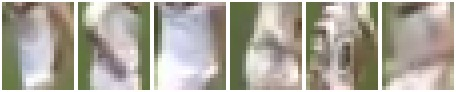
\includegraphics[width=39mm]{refchips_target.jpg}};
  \node[below=4mm of clu, xshift=21.5mm, anchor=north, inner sep=0] (oth)
       {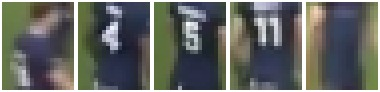
\includegraphics[width=33mm]{refchips_other.jpg}};
  \node[below=0.5mm of tgt, font=\tiny] {target-cluster reference crops};
  \node[below=0.5mm of oth, font=\tiny] {opponent-cluster reference crops};
  \draw[arr] (clu.south) ++(-21.5mm,0) -- (tgt.north);
  \draw[arr] (clu.south) ++(21.5mm,0) -- (oth.north);

  % output
  \node[stud, below=13mm of clu, text width=56mm, yshift=-8mm]
       (refs) {per-team colour histogram $+$ embedding centroid;\\
               fusion weights learned automatically\\
               ($w_{\text{colour}} \approx 0.48$--$0.53$ across deployment matches)};
  \draw[arr] (tgt.south) ++(0,-3.5mm) -- (refs.north -| tgt.south);
  \draw[arr] (oth.south) ++(0,-3.5mm) -- (refs.north -| oth.south);
\end{tikzpicture}

\caption{\textbf{Zero-manual-setup team-reference bootstrap (C2).} A three-tier
cascade selects which cluster of jersey crops is the target team; the chosen
clusters become per-team references (colour histogram $+$ vision-embedding
centroid) with fusion weights learned automatically. Crops shown are an
illustrative reconstruction on one daylight fixture using the same
detect--crop--cluster procedure; they are torso-only and deliberately pixelated,
since the deployed system stores only the resulting feature centroids, never
images.}
\label{fig:teamref}
\end{figure}
Each detected logo instance is then attributed to the team of its nearest tracked
person. When the evidence for opponent ownership is insufficient (a track has not yet
accumulated enough confident votes), the instance is \emph{kept} rather than dropped —
an explicit, revenue-safe design choice: an under-confident drop would silently
understate a paying sponsor's measured exposure, which we consider a worse failure mode
than a small number of false positives that a human reviewer can catch.

\subsection{Visibility, exposure, and EMV pricing}
\label{sec:emv}
Exposure and pricing are computed in three tiers, adapted from the manual AVE/EMV family
discussed in \S\ref{sec:related-pricing} rather than proposed as a new pricing theory:
(1) a per-frame \emph{visibility} score combining detection size, on-screen position,
and detector confidence; (2) temporal aggregation of visibility into per-brand
\emph{exposure} segments, discarding very short, likely spurious detections; and (3) a
conversion to \emph{estimated media value} using an audience size, a cost-per-thousand
(CPM) baseline, and a placement multiplier supplied per deployment (the implementation
additionally supports sponsor-category and prime-time multipliers, both disabled in the
deployment reported here). A specific
calibration lesson from deployment: the visibility floor of 0.1 suggested in the
pricing methodology we adapt, applied as published, discards nearly all real, small,
off-centre sponsor logos typical of kit sponsorship — under our size term such logos
score in the 0.03--0.08 range — so we use an empirically set floor of 0.02
(\TODOnum{report the sensitivity of exposure-seconds to this visibility floor and to
the detector confidence floor of 0.25 jointly}).

\subsection{Placement-level pricing}
Each attributed detection is additionally assigned to one of eighteen kit slots (e.g.\
chest-centre, sleeve, sock) via pose-estimation keypoints, so that exposure — and hence
the placement multiplier applied in Tier 3 — can be reported and priced per slot rather
than only per brand (the measured per-slot distribution from our deployment is shown in
Fig.~\ref{fig:kitslots}). This directly targets the ``arbitrary multiplier'' criticism of
AVE-style pricing (\S\ref{sec:related-pricing}) by grounding part of the multiplier in
measured, slot-specific exposure share, while leaving audience-quality and sentiment
signals as future work (\S\ref{sec:discussion}).

% ============================================================================
\section{Experiments}
\label{sec:exp}

\subsection{Setup}
We evaluate on match video self-ingested by our partner club (identity withheld) —
video the club captured and uploaded itself, not an official broadcast feed. The
annotated detection dataset covers seventeen sponsor classes and is severely
imbalanced, from roughly 200 instances for the most frequent kit sponsor down to
single digits for the rarest — a property of real kit sponsorship, not of our
sampling, since a chest sponsor simply appears in almost every frame while a
shorts-leg sponsor does not. Detector
training and evaluation use a clip-disjoint split: all frames from the same clip or
match are kept entirely within one split. This choice matters more than any
architectural one we made: because analytics frames are sampled at 2\,fps,
neighbouring frames are near-duplicates, and a naive random-frame split leaks them
across train and validation. The same YOLO26m detector scores mAP@0.5 = 0.86 under a
random-frame split but 0.70 under the clip-disjoint split of the same source data
(Table~\ref{tab:split}) —
the higher number reflects leakage, not a better model, and we report the pair
explicitly because published results in this domain rarely state which split
strategy was used.

\begin{table}[t]
\centering
\caption{Effect of the train/validation split policy on measured detection accuracy
(fine-tuned YOLO26m, best validation epoch). The random-frame figure is inflated by
near-duplicate frames leaking across the split, not by a better model.}
\label{tab:split}
\begin{tabular}{lcc}
\toprule
Split policy & mAP@0.5 & mAP@[.5:.95] \\
\midrule
Random-frame                  & 0.86 & 0.57 \\
Clip-disjoint, same data      & 0.70 & 0.42 \\
Clip-disjoint, extended data  & \textbf{0.75} & \textbf{0.44} \\
\bottomrule
\end{tabular}
\end{table}

\subsection{Detection accuracy}
On the initial annotated set, the clip-disjoint validation score is mAP@0.5 = 0.70
(mAP@[.5:.95] = 0.42); after extending the dataset with additional annotated clips
under the same clip-aware split policy, the current detector reaches mAP@0.5 = 0.75
(mAP@[.5:.95] = 0.44, precision 0.65, recall 0.74). Rare-class AP is unreliable at
these instance counts and the validation split intentionally holds no instances of
the rarest classes, so aggregate mAP should be read together with the per-class
breakdown.

\begin{figure}[!t]
\centering
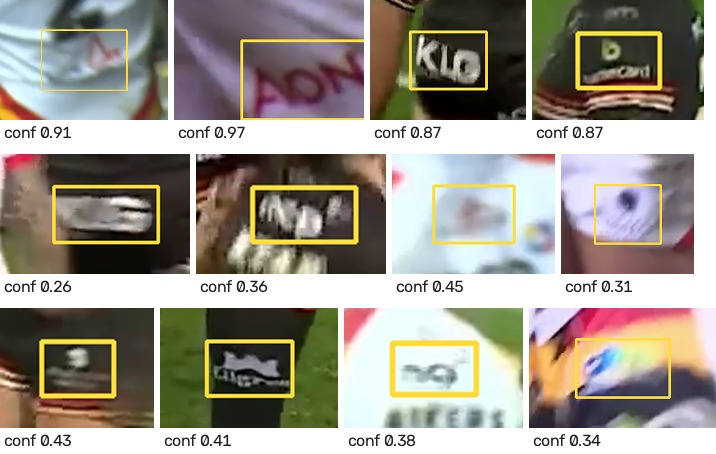
\includegraphics[width=\linewidth]{hard_examples.jpg}
\caption{\textbf{The detection-confidence spectrum in self-captured video} (boxes;
confidence under each crop) from one night and one daylight fixture. Top row:
representative high-confidence detections (0.87--0.97) — sharp, large, frontal marks;
in deployment this regime carries 64\% of quality-weighted exposure. Lower rows: the
hard tail — floodlit night play, heavy motion blur, sub-0.1\%-of-frame scale, and
fold/occlusion deformation — which is routine in club-captured footage. Marks in the
hard tail are inherently illegible at capture, which is precisely why a hard
confidence gate would delete genuine exposure; the pipeline keeps them and lets
visibility weighting and the minimum-duration rule (\S\ref{sec:emv}) suppress
spurious ones.}
\label{fig:hard}
\end{figure}

Three observations frame whether 0.75 is ``enough.'' First, the operating domain is
harder than professionally produced broadcast: Fig.~\ref{fig:hard} spans the
confidence spectrum the detector produces on this footage — most exposure comes from
clean, high-confidence detections, but a hard tail of small, motion-blurred, deformed
marks is routine in club-captured video and drags aggregate mAP in a way that clean
broadcast benchmarks never see. Second, the number is not comparable to
published results unless the split protocol is stated: our own detector reaches 0.86
when near-duplicate frames leak across the split (Table~\ref{tab:split}), so a
protocol-silent comparison against, e.g., ExposureEngine's
0.859~\cite{exposureengine} — reported on broadcast footage,
a different domain — would be meaningless in either
direction. Third, per-frame mAP is not the quantity a sponsor report is built from.
Exposure is computed from temporally aggregated segments (\S\ref{sec:emv}): the gap
tolerance bridges isolated per-frame misses within a segment, and the
minimum-duration rule discards isolated false positives, so moderate per-frame
accuracy on a tracked, repeatedly visible logo can still yield accurate
exposure-seconds. The operative accuracy metric for the system's end output is
therefore the exposure-seconds error against manual timing (\S\ref{sec:exp}, EMV
validation), with mAP reported for completeness and future comparability. \TODOnum{Report per-class average precision and a confusion matrix on a
held-out clip-disjoint test split (current numbers are validation-split figures used
for model selection).}

\subsection{Team attribution}
\TODOnum{Report precision/recall of team attribution on a labelled clip sample spanning
more than one match and lighting condition (current evidence: two case-study clips only
— insufficient for a quantitative claim and must be extended before submission).}

\subsection{Team-attribution counterfactual}
\label{sec:exp-counterfactual}
Across nine full-match highlight videos processed by the deployed pipeline, team
attribution flagged and excluded 44\% of raw logo detections (11{,}161 of 25{,}153)
as owned by the opposing team or match officials, or as not attached to any tracked
player (e.g.\ perimeter advertising boards). We did not take this aggregate at face
value: we visually audited the per-track attribution overlays of all nine matches.
Five show correct target/opponent assignment; three (two night-time,
long-range club-feed fixtures and one fixture in which both teams wore dark kits)
work overall but exhibit per-track errors in both directions; and in one — the
match with the highest exclusion rate, 78\% — the fused classifier systematically
assigned the target club's own white kit to the opponent class under night
floodlighting, despite reference features that a luminance check confirms are
correct. We report that last match as a failure case (\S\ref{sec:discussion}), not
as filtering, and exclude it from the headline figure: over the remaining eight
matches, attribution excluded 41\% of raw detections (9{,}383 of 22{,}863), with
per-match rates of 21--50\% on dark-kit fixtures and 26--72\% on white-kit fixtures
— the upper end driven by the noisy night-time captures above, in which many distant
tracks never accumulate a confident label. Without attribution, every excluded detection would have been counted —
and priced — as target-club kit exposure. These figures quantify how much raw
exposure the filter removes in production, not yet its per-instance accuracy, which
is the subject of the labelled-clip evaluation of the previous subsection. To isolate
the value of C1 further, we additionally run the pipeline with team attribution
enabled and disabled on clips where a sponsor appears on both teams' kits, and report
the resulting difference in measured exposure-seconds and EMV.
\TODOnum{Report the counterfactual over-counting avoided on shared-sponsor clips,
e.g.\ ``X\% lower EMV / correctly attributed exposure-seconds with team attribution
on.''}

\begin{figure*}[t]
\centering
\resizebox{\textwidth}{!}{% Auto-generated from backend/data/app.db (analysis e6d8bf5d7eb8, M04 black-kit
% full-highlight video, 533.7 s). Regenerate with scratchpad gen_paper_figs.py.
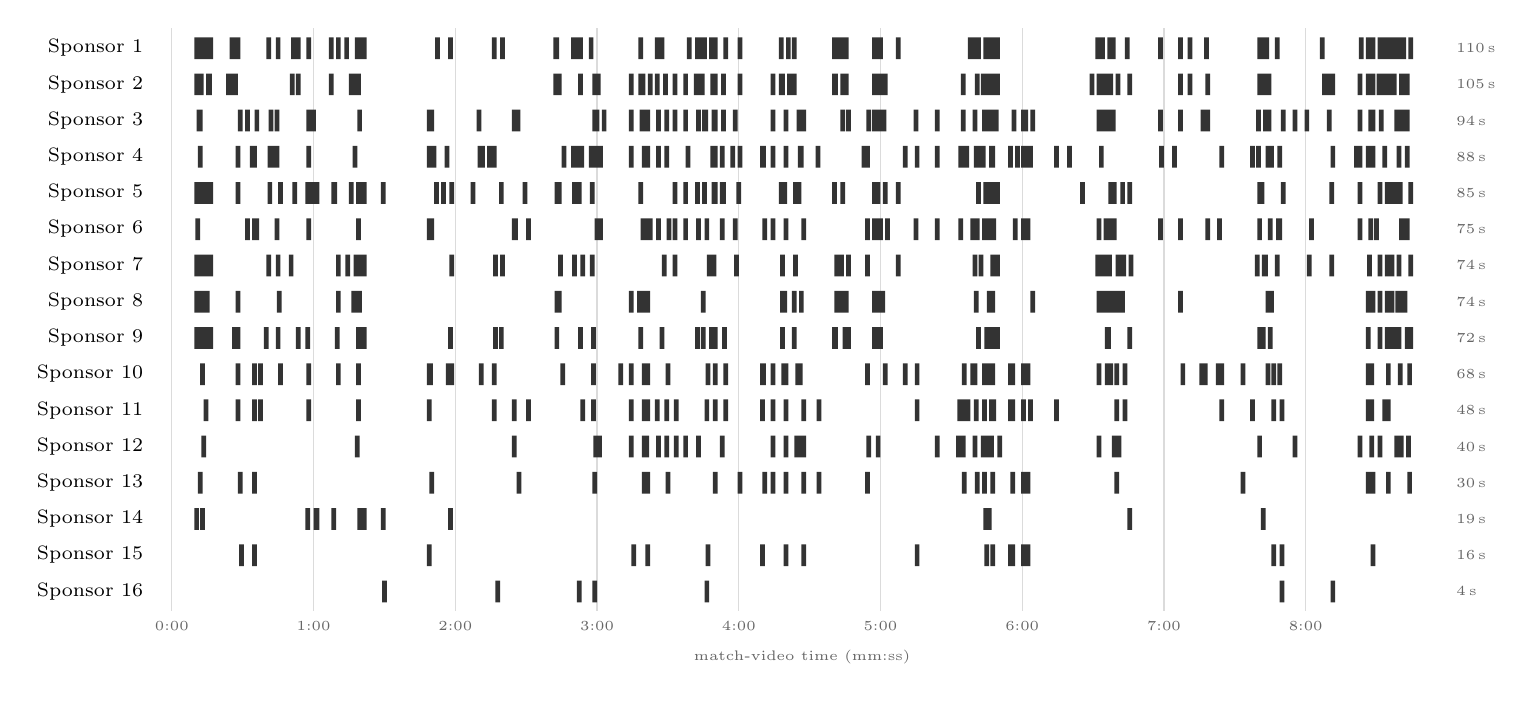
\begin{tikzpicture}[x=0.30mm, y=-4.6mm]
  % recessive time grid (every 60 s) + labels
  \draw[black!14, line width=0.4pt] (0,-0.55) -- (0,15.55);
  \node[font=\tiny, text=black!60, anchor=north] at (0,15.55) {0:00};
  \draw[black!14, line width=0.4pt] (60,-0.55) -- (60,15.55);
  \node[font=\tiny, text=black!60, anchor=north] at (60,15.55) {1:00};
  \draw[black!14, line width=0.4pt] (120,-0.55) -- (120,15.55);
  \node[font=\tiny, text=black!60, anchor=north] at (120,15.55) {2:00};
  \draw[black!14, line width=0.4pt] (180,-0.55) -- (180,15.55);
  \node[font=\tiny, text=black!60, anchor=north] at (180,15.55) {3:00};
  \draw[black!14, line width=0.4pt] (240,-0.55) -- (240,15.55);
  \node[font=\tiny, text=black!60, anchor=north] at (240,15.55) {4:00};
  \draw[black!14, line width=0.4pt] (300,-0.55) -- (300,15.55);
  \node[font=\tiny, text=black!60, anchor=north] at (300,15.55) {5:00};
  \draw[black!14, line width=0.4pt] (360,-0.55) -- (360,15.55);
  \node[font=\tiny, text=black!60, anchor=north] at (360,15.55) {6:00};
  \draw[black!14, line width=0.4pt] (420,-0.55) -- (420,15.55);
  \node[font=\tiny, text=black!60, anchor=north] at (420,15.55) {7:00};
  \draw[black!14, line width=0.4pt] (480,-0.55) -- (480,15.55);
  \node[font=\tiny, text=black!60, anchor=north] at (480,15.55) {8:00};
  \node[font=\tiny, text=black!60, anchor=north] at (266.85,16.35) {match-video time (mm:ss)};
  % one row per sponsor, sorted by total on-screen time
  \node[font=\scriptsize, anchor=east] at (-8,0) {Sponsor 1};
  \fill[black!80] (9.5,-0.3) rectangle (17.5,0.3) (24.5,-0.3) rectangle (26.5,0.3) (26.5,-0.3) rectangle (29.0,0.3) (40.0,-0.3) rectangle (42.0,0.3) (44.0,-0.3) rectangle (46.0,0.3) (50.5,-0.3) rectangle (52.5,0.3) (52.5,-0.3) rectangle (54.5,0.3) (57.0,-0.3) rectangle (59.0,0.3) (66.5,-0.3) rectangle (68.5,0.3) (69.5,-0.3) rectangle (71.5,0.3) (73.0,-0.3) rectangle (75.0,0.3) (77.5,-0.3) rectangle (82.5,0.3) (111.5,-0.3) rectangle (113.5,0.3) (117.0,-0.3) rectangle (119.0,0.3) (135.5,-0.3) rectangle (137.5,0.3) (139.0,-0.3) rectangle (141.0,0.3) (161.5,-0.3) rectangle (164.0,0.3) (169.0,-0.3) rectangle (174.0,0.3) (176.5,-0.3) rectangle (178.5,0.3) (197.5,-0.3) rectangle (199.5,0.3) (204.5,-0.3) rectangle (206.5,0.3) (206.5,-0.3) rectangle (208.5,0.3) (218.0,-0.3) rectangle (220.0,0.3) (221.5,-0.3) rectangle (223.5,0.3) (223.5,-0.3) rectangle (226.5,0.3) (227.5,-0.3) rectangle (231.0,0.3) (233.5,-0.3) rectangle (235.5,0.3) (239.5,-0.3) rectangle (241.5,0.3) (257.0,-0.3) rectangle (259.0,0.3) (260.0,-0.3) rectangle (262.0,0.3) (262.5,-0.3) rectangle (264.5,0.3) (279.5,-0.3) rectangle (286.5,0.3) (296.5,-0.3) rectangle (301.0,0.3) (306.5,-0.3) rectangle (308.5,0.3) (337.0,-0.3) rectangle (339.0,0.3) (339.0,-0.3) rectangle (342.5,0.3) (343.5,-0.3) rectangle (350.5,0.3) (391.0,-0.3) rectangle (393.0,0.3) (393.0,-0.3) rectangle (395.0,0.3) (396.0,-0.3) rectangle (399.5,0.3) (403.5,-0.3) rectangle (405.5,0.3) (417.5,-0.3) rectangle (419.5,0.3) (426.0,-0.3) rectangle (428.0,0.3) (430.0,-0.3) rectangle (432.0,0.3) (437.0,-0.3) rectangle (439.0,0.3) (459.5,-0.3) rectangle (464.5,0.3) (467.0,-0.3) rectangle (469.0,0.3) (486.0,-0.3) rectangle (488.0,0.3) (502.5,-0.3) rectangle (504.5,0.3) (505.5,-0.3) rectangle (507.5,0.3) (507.5,-0.3) rectangle (509.5,0.3) (510.5,-0.3) rectangle (522.5,0.3) (523.5,-0.3) rectangle (525.5,0.3);
  \node[font=\tiny, text=black!60, anchor=west] at (539.7,0) {110\,s};
  \node[font=\scriptsize, anchor=east] at (-8,1) {Sponsor 2};
  \fill[black!80] (9.5,0.7) rectangle (13.5,1.3) (14.5,0.7) rectangle (17.0,1.3) (23.0,0.7) rectangle (25.0,1.3) (24.5,0.7) rectangle (28.0,1.3) (50.0,0.7) rectangle (52.0,1.3) (52.5,0.7) rectangle (54.5,1.3) (66.5,0.7) rectangle (68.5,1.3) (75.0,0.7) rectangle (80.0,1.3) (161.5,0.7) rectangle (165.0,1.3) (172.0,0.7) rectangle (174.0,1.3) (178.0,0.7) rectangle (181.5,1.3) (193.5,0.7) rectangle (195.5,1.3) (197.5,0.7) rectangle (200.5,1.3) (201.5,0.7) rectangle (203.5,1.3) (204.5,0.7) rectangle (206.5,1.3) (208.0,0.7) rectangle (210.0,1.3) (212.0,0.7) rectangle (214.0,1.3) (216.5,0.7) rectangle (218.5,1.3) (221.0,0.7) rectangle (225.5,1.3) (228.0,0.7) rectangle (231.0,1.3) (232.5,0.7) rectangle (234.5,1.3) (239.5,0.7) rectangle (241.5,1.3) (253.5,0.7) rectangle (255.5,1.3) (257.0,0.7) rectangle (259.5,1.3) (260.5,0.7) rectangle (262.5,1.3) (262.5,0.7) rectangle (264.5,1.3) (279.5,0.7) rectangle (282.0,1.3) (283.0,0.7) rectangle (286.5,1.3) (296.5,0.7) rectangle (303.0,1.3) (334.0,0.7) rectangle (336.0,1.3) (340.0,0.7) rectangle (342.0,1.3) (342.5,0.7) rectangle (350.5,1.3) (388.5,0.7) rectangle (390.5,1.3) (391.5,0.7) rectangle (398.5,1.3) (399.5,0.7) rectangle (401.5,1.3) (404.5,0.7) rectangle (406.5,1.3) (426.0,0.7) rectangle (428.0,1.3) (430.0,0.7) rectangle (432.0,1.3) (437.5,0.7) rectangle (439.5,1.3) (459.5,0.7) rectangle (461.5,1.3) (461.5,0.7) rectangle (463.5,1.3) (463.0,0.7) rectangle (465.5,1.3) (487.0,0.7) rectangle (489.0,1.3) (489.0,0.7) rectangle (491.0,1.3) (490.5,0.7) rectangle (492.5,1.3) (502.0,0.7) rectangle (504.0,1.3) (505.5,0.7) rectangle (507.5,1.3) (507.5,0.7) rectangle (509.5,1.3) (510.0,0.7) rectangle (518.5,1.3) (519.5,0.7) rectangle (524.0,1.3);
  \node[font=\tiny, text=black!60, anchor=west] at (539.7,1) {105\,s};
  \node[font=\scriptsize, anchor=east] at (-8,2) {Sponsor 3};
  \fill[black!80] (10.5,1.7) rectangle (13.0,2.3) (28.0,1.7) rectangle (30.0,2.3) (31.0,1.7) rectangle (33.0,2.3) (35.0,1.7) rectangle (37.0,2.3) (41.0,1.7) rectangle (43.0,2.3) (43.5,1.7) rectangle (45.5,2.3) (57.0,1.7) rectangle (59.0,2.3) (59.0,1.7) rectangle (61.0,2.3) (78.5,1.7) rectangle (80.5,2.3) (108.0,1.7) rectangle (111.0,2.3) (129.0,1.7) rectangle (131.0,2.3) (144.0,1.7) rectangle (146.0,2.3) (145.5,1.7) rectangle (147.5,2.3) (178.0,1.7) rectangle (181.0,2.3) (182.0,1.7) rectangle (184.0,2.3) (193.5,1.7) rectangle (195.5,2.3) (198.0,1.7) rectangle (202.5,2.3) (205.0,1.7) rectangle (207.0,2.3) (208.5,1.7) rectangle (210.5,2.3) (212.0,1.7) rectangle (214.0,2.3) (216.5,1.7) rectangle (218.5,2.3) (222.0,1.7) rectangle (224.0,2.3) (224.5,1.7) rectangle (227.0,2.3) (228.5,1.7) rectangle (231.0,2.3) (232.5,1.7) rectangle (234.5,2.3) (237.5,1.7) rectangle (239.5,2.3) (253.5,1.7) rectangle (255.5,2.3) (259.0,1.7) rectangle (261.0,2.3) (264.5,1.7) rectangle (266.5,2.3) (266.5,1.7) rectangle (268.5,2.3) (283.0,1.7) rectangle (285.0,2.3) (285.5,1.7) rectangle (287.5,2.3) (294.0,1.7) rectangle (296.0,2.3) (296.5,1.7) rectangle (302.5,2.3) (314.0,1.7) rectangle (316.0,2.3) (323.0,1.7) rectangle (325.0,2.3) (334.0,1.7) rectangle (336.0,2.3) (339.0,1.7) rectangle (341.0,2.3) (343.0,1.7) rectangle (350.0,2.3) (355.5,1.7) rectangle (357.5,2.3) (359.5,1.7) rectangle (362.5,2.3) (363.5,1.7) rectangle (365.5,2.3) (391.5,1.7) rectangle (399.5,2.3) (417.5,1.7) rectangle (419.5,2.3) (426.0,1.7) rectangle (428.0,2.3) (435.5,1.7) rectangle (437.5,2.3) (437.5,1.7) rectangle (439.5,2.3) (459.0,1.7) rectangle (461.0,2.3) (462.0,1.7) rectangle (464.0,2.3) (463.5,1.7) rectangle (465.5,2.3) (469.5,1.7) rectangle (471.5,2.3) (474.5,1.7) rectangle (476.5,2.3) (479.5,1.7) rectangle (481.5,2.3) (489.0,1.7) rectangle (491.0,2.3) (502.0,1.7) rectangle (504.0,2.3) (506.5,1.7) rectangle (509.5,2.3) (511.0,1.7) rectangle (513.0,2.3) (517.5,1.7) rectangle (524.0,2.3);
  \node[font=\tiny, text=black!60, anchor=west] at (539.7,2) {94\,s};
  \node[font=\scriptsize, anchor=east] at (-8,3) {Sponsor 4};
  \fill[black!80] (11.0,2.7) rectangle (13.0,3.3) (27.0,2.7) rectangle (29.0,3.3) (33.0,2.7) rectangle (36.0,3.3) (40.5,2.7) rectangle (42.5,3.3) (42.0,2.7) rectangle (44.0,3.3) (43.5,2.7) rectangle (45.5,3.3) (57.0,2.7) rectangle (59.0,3.3) (76.5,2.7) rectangle (78.5,3.3) (108.0,2.7) rectangle (110.0,3.3) (110.0,2.7) rectangle (112.0,3.3) (115.5,2.7) rectangle (117.5,3.3) (129.5,2.7) rectangle (132.5,3.3) (133.5,2.7) rectangle (135.5,3.3) (135.5,2.7) rectangle (137.5,3.3) (165.0,2.7) rectangle (167.0,3.3) (169.0,2.7) rectangle (174.5,3.3) (176.5,2.7) rectangle (182.5,3.3) (193.5,2.7) rectangle (195.5,3.3) (199.0,2.7) rectangle (202.5,3.3) (205.0,2.7) rectangle (207.0,3.3) (208.5,2.7) rectangle (210.5,3.3) (217.5,2.7) rectangle (219.5,3.3) (228.0,2.7) rectangle (231.0,3.3) (232.0,2.7) rectangle (234.0,3.3) (236.5,2.7) rectangle (238.5,3.3) (239.5,2.7) rectangle (241.5,3.3) (249.0,2.7) rectangle (251.5,3.3) (253.5,2.7) rectangle (255.5,3.3) (259.0,2.7) rectangle (261.0,3.3) (265.0,2.7) rectangle (267.5,3.3) (272.5,2.7) rectangle (274.5,3.3) (292.0,2.7) rectangle (294.0,3.3) (293.5,2.7) rectangle (295.5,3.3) (309.5,2.7) rectangle (311.5,3.3) (314.5,2.7) rectangle (316.5,3.3) (323.0,2.7) rectangle (325.0,3.3) (333.0,2.7) rectangle (337.5,3.3) (339.5,2.7) rectangle (344.5,3.3) (346.0,2.7) rectangle (348.5,3.3) (354.0,2.7) rectangle (356.0,3.3) (357.0,2.7) rectangle (359.0,3.3) (359.5,2.7) rectangle (361.5,3.3) (361.0,2.7) rectangle (364.5,3.3) (373.5,2.7) rectangle (375.5,3.3) (379.0,2.7) rectangle (381.0,3.3) (392.5,2.7) rectangle (394.5,3.3) (418.0,2.7) rectangle (420.0,3.3) (423.5,2.7) rectangle (425.5,3.3) (443.5,2.7) rectangle (445.5,3.3) (456.5,2.7) rectangle (458.5,3.3) (459.0,2.7) rectangle (461.0,3.3) (463.0,2.7) rectangle (465.0,3.3) (464.5,2.7) rectangle (466.5,3.3) (468.0,2.7) rectangle (470.0,3.3) (490.5,2.7) rectangle (492.5,3.3) (500.5,2.7) rectangle (502.5,3.3) (502.0,2.7) rectangle (504.0,3.3) (505.5,2.7) rectangle (509.5,3.3) (512.5,2.7) rectangle (514.5,3.3) (518.5,2.7) rectangle (520.5,3.3) (522.0,2.7) rectangle (524.0,3.3);
  \node[font=\tiny, text=black!60, anchor=west] at (539.7,3) {88\,s};
  \node[font=\scriptsize, anchor=east] at (-8,4) {Sponsor 5};
  \fill[black!80] (9.5,3.7) rectangle (17.5,4.3) (27.0,3.7) rectangle (29.0,4.3) (40.5,3.7) rectangle (42.5,4.3) (45.0,3.7) rectangle (47.0,4.3) (51.0,3.7) rectangle (53.0,4.3) (56.5,3.7) rectangle (58.5,4.3) (58.0,3.7) rectangle (60.0,4.3) (60.0,3.7) rectangle (62.5,4.3) (67.5,3.7) rectangle (70.0,4.3) (75.0,3.7) rectangle (77.0,4.3) (78.0,3.7) rectangle (82.5,4.3) (88.5,3.7) rectangle (90.5,4.3) (111.0,3.7) rectangle (113.0,4.3) (114.0,3.7) rectangle (116.0,4.3) (117.5,3.7) rectangle (119.5,4.3) (126.5,3.7) rectangle (128.5,4.3) (138.5,3.7) rectangle (140.5,4.3) (148.5,3.7) rectangle (150.5,4.3) (162.0,3.7) rectangle (165.0,4.3) (169.5,3.7) rectangle (171.5,4.3) (171.5,3.7) rectangle (173.5,4.3) (177.0,3.7) rectangle (179.0,4.3) (197.5,3.7) rectangle (199.5,4.3) (212.0,3.7) rectangle (214.0,4.3) (216.5,3.7) rectangle (218.5,4.3) (221.5,3.7) rectangle (223.5,4.3) (224.5,3.7) rectangle (226.5,4.3) (228.5,3.7) rectangle (231.0,4.3) (232.0,3.7) rectangle (234.5,4.3) (239.0,3.7) rectangle (241.0,4.3) (257.0,3.7) rectangle (260.5,4.3) (263.0,3.7) rectangle (265.0,4.3) (264.5,3.7) rectangle (266.5,4.3) (279.5,3.7) rectangle (281.5,4.3) (283.0,3.7) rectangle (285.0,4.3) (296.5,3.7) rectangle (300.0,4.3) (301.0,3.7) rectangle (303.0,4.3) (306.5,3.7) rectangle (308.5,4.3) (340.5,3.7) rectangle (342.5,4.3) (343.5,3.7) rectangle (350.5,4.3) (384.5,3.7) rectangle (386.5,4.3) (396.5,3.7) rectangle (398.5,4.3) (398.0,3.7) rectangle (400.0,4.3) (401.5,3.7) rectangle (403.5,4.3) (404.5,3.7) rectangle (406.5,4.3) (459.5,3.7) rectangle (462.5,4.3) (469.5,3.7) rectangle (471.5,4.3) (490.0,3.7) rectangle (492.0,4.3) (502.0,3.7) rectangle (504.0,4.3) (510.5,3.7) rectangle (512.5,4.3) (513.5,3.7) rectangle (521.0,4.3) (523.5,3.7) rectangle (525.5,4.3);
  \node[font=\tiny, text=black!60, anchor=west] at (539.7,4) {85\,s};
  \node[font=\scriptsize, anchor=east] at (-8,5) {Sponsor 6};
  \fill[black!80] (10.0,4.7) rectangle (12.0,5.3) (31.0,4.7) rectangle (33.0,5.3) (34.0,4.7) rectangle (37.0,5.3) (43.5,4.7) rectangle (45.5,5.3) (57.0,4.7) rectangle (59.0,5.3) (78.0,4.7) rectangle (80.0,5.3) (108.0,4.7) rectangle (111.0,5.3) (144.0,4.7) rectangle (146.5,5.3) (150.0,4.7) rectangle (152.0,5.3) (179.0,4.7) rectangle (182.5,5.3) (198.5,4.7) rectangle (200.5,5.3) (200.0,4.7) rectangle (202.0,5.3) (201.5,4.7) rectangle (203.5,5.3) (205.0,4.7) rectangle (207.0,5.3) (209.5,4.7) rectangle (211.5,5.3) (212.0,4.7) rectangle (214.0,5.3) (216.5,4.7) rectangle (218.5,5.3) (222.0,4.7) rectangle (224.0,5.3) (225.5,4.7) rectangle (227.5,5.3) (232.0,4.7) rectangle (234.0,5.3) (237.5,4.7) rectangle (239.5,5.3) (250.0,4.7) rectangle (252.0,5.3) (253.5,4.7) rectangle (255.5,5.3) (259.0,4.7) rectangle (261.0,5.3) (266.5,4.7) rectangle (268.5,5.3) (293.5,4.7) rectangle (295.5,5.3) (296.5,4.7) rectangle (301.0,5.3) (302.0,4.7) rectangle (304.0,5.3) (314.0,4.7) rectangle (316.0,5.3) (323.0,4.7) rectangle (325.0,5.3) (333.0,4.7) rectangle (335.0,5.3) (338.0,4.7) rectangle (340.0,5.3) (340.0,4.7) rectangle (342.0,5.3) (343.0,4.7) rectangle (349.0,5.3) (356.0,4.7) rectangle (358.0,5.3) (359.5,4.7) rectangle (363.5,5.3) (391.5,4.7) rectangle (393.5,5.3) (394.5,4.7) rectangle (400.0,5.3) (417.5,4.7) rectangle (419.5,5.3) (426.0,4.7) rectangle (428.0,5.3) (437.5,4.7) rectangle (439.5,5.3) (442.5,4.7) rectangle (444.5,5.3) (459.5,4.7) rectangle (461.5,5.3) (464.0,4.7) rectangle (466.0,5.3) (467.5,4.7) rectangle (470.0,5.3) (481.5,4.7) rectangle (483.5,5.3) (502.0,4.7) rectangle (504.0,5.3) (506.5,4.7) rectangle (508.5,5.3) (509.0,4.7) rectangle (511.0,5.3) (519.5,4.7) rectangle (524.0,5.3);
  \node[font=\tiny, text=black!60, anchor=west] at (539.7,5) {75\,s};
  \node[font=\scriptsize, anchor=east] at (-8,6) {Sponsor 7};
  \fill[black!80] (9.5,5.7) rectangle (17.5,6.3) (40.0,5.7) rectangle (42.0,6.3) (44.0,5.7) rectangle (46.0,6.3) (49.5,5.7) rectangle (51.5,6.3) (69.5,5.7) rectangle (71.5,6.3) (73.5,5.7) rectangle (75.5,6.3) (77.0,5.7) rectangle (82.5,6.3) (117.5,5.7) rectangle (119.5,6.3) (136.0,5.7) rectangle (138.0,6.3) (139.0,5.7) rectangle (141.0,6.3) (163.5,5.7) rectangle (165.5,6.3) (169.5,5.7) rectangle (171.5,6.3) (173.0,5.7) rectangle (175.0,6.3) (177.0,5.7) rectangle (179.0,6.3) (207.5,5.7) rectangle (209.5,6.3) (212.0,5.7) rectangle (214.0,6.3) (226.5,5.7) rectangle (230.5,6.3) (238.0,5.7) rectangle (240.0,6.3) (257.5,5.7) rectangle (259.5,6.3) (263.0,5.7) rectangle (265.0,6.3) (280.5,5.7) rectangle (284.5,6.3) (285.5,5.7) rectangle (287.5,6.3) (293.5,5.7) rectangle (295.5,6.3) (306.5,5.7) rectangle (308.5,6.3) (339.0,5.7) rectangle (341.0,6.3) (341.5,5.7) rectangle (343.5,6.3) (346.5,5.7) rectangle (350.5,6.3) (391.0,5.7) rectangle (398.0,6.3) (399.5,5.7) rectangle (404.0,6.3) (405.0,5.7) rectangle (407.0,6.3) (458.5,5.7) rectangle (460.5,6.3) (461.5,5.7) rectangle (464.0,6.3) (467.0,5.7) rectangle (469.0,6.3) (480.5,5.7) rectangle (482.5,6.3) (490.0,5.7) rectangle (492.0,6.3) (506.0,5.7) rectangle (508.0,6.3) (510.5,5.7) rectangle (512.5,6.3) (513.5,5.7) rectangle (517.5,6.3) (518.5,5.7) rectangle (520.5,6.3) (523.5,5.7) rectangle (525.5,6.3);
  \node[font=\tiny, text=black!60, anchor=west] at (539.7,6) {74\,s};
  \node[font=\scriptsize, anchor=east] at (-8,7) {Sponsor 8};
  \fill[black!80] (9.5,6.7) rectangle (11.5,7.3) (11.0,6.7) rectangle (16.0,7.3) (27.0,6.7) rectangle (29.0,7.3) (44.5,6.7) rectangle (46.5,7.3) (69.5,6.7) rectangle (71.5,7.3) (76.0,6.7) rectangle (80.5,7.3) (162.0,6.7) rectangle (165.0,7.3) (193.5,6.7) rectangle (195.5,7.3) (197.0,6.7) rectangle (202.5,7.3) (224.0,6.7) rectangle (226.0,7.3) (257.5,6.7) rectangle (260.5,7.3) (262.5,6.7) rectangle (264.5,7.3) (265.5,6.7) rectangle (267.5,7.3) (280.5,6.7) rectangle (286.5,7.3) (296.5,6.7) rectangle (302.0,7.3) (339.5,6.7) rectangle (341.5,7.3) (345.0,6.7) rectangle (348.5,7.3) (363.5,6.7) rectangle (365.5,7.3) (391.5,6.7) rectangle (403.5,7.3) (426.0,6.7) rectangle (428.0,7.3) (463.0,6.7) rectangle (465.0,7.3) (464.5,6.7) rectangle (466.5,7.3) (505.5,6.7) rectangle (509.5,7.3) (510.5,6.7) rectangle (512.5,7.3) (513.5,6.7) rectangle (515.5,7.3) (515.5,6.7) rectangle (517.5,7.3) (518.0,6.7) rectangle (523.0,7.3);
  \node[font=\tiny, text=black!60, anchor=west] at (539.7,7) {74\,s};
  \node[font=\scriptsize, anchor=east] at (-8,8) {Sponsor 9};
  \fill[black!80] (9.5,7.7) rectangle (17.5,8.3) (25.5,7.7) rectangle (27.5,8.3) (27.0,7.7) rectangle (29.0,8.3) (39.0,7.7) rectangle (41.0,8.3) (44.0,7.7) rectangle (46.0,8.3) (52.5,7.7) rectangle (54.5,8.3) (56.5,7.7) rectangle (58.5,8.3) (69.0,7.7) rectangle (71.0,8.3) (78.0,7.7) rectangle (82.5,8.3) (117.0,7.7) rectangle (119.0,8.3) (136.0,7.7) rectangle (138.0,8.3) (138.5,7.7) rectangle (140.5,8.3) (162.0,7.7) rectangle (164.0,8.3) (172.0,7.7) rectangle (174.0,8.3) (177.5,7.7) rectangle (179.5,8.3) (197.5,7.7) rectangle (199.5,8.3) (206.5,7.7) rectangle (208.5,8.3) (221.5,7.7) rectangle (223.5,8.3) (224.0,7.7) rectangle (226.0,8.3) (227.5,7.7) rectangle (229.5,8.3) (229.0,7.7) rectangle (231.0,8.3) (233.0,7.7) rectangle (235.0,8.3) (257.5,7.7) rectangle (259.5,8.3) (262.5,7.7) rectangle (264.5,8.3) (279.5,7.7) rectangle (282.0,8.3) (284.0,7.7) rectangle (286.0,8.3) (285.5,7.7) rectangle (287.5,8.3) (296.5,7.7) rectangle (301.0,8.3) (340.5,7.7) rectangle (342.5,8.3) (344.0,7.7) rectangle (350.5,8.3) (395.0,7.7) rectangle (397.5,8.3) (404.5,7.7) rectangle (406.5,8.3) (459.5,7.7) rectangle (463.0,8.3) (464.0,7.7) rectangle (466.0,8.3) (505.5,7.7) rectangle (507.5,8.3) (510.5,7.7) rectangle (512.5,8.3) (513.5,7.7) rectangle (520.5,8.3) (522.0,7.7) rectangle (524.0,8.3) (523.5,7.7) rectangle (525.5,8.3);
  \node[font=\tiny, text=black!60, anchor=west] at (539.7,8) {72\,s};
  \node[font=\scriptsize, anchor=east] at (-8,9) {Sponsor 10};
  \fill[black!80] (12.0,8.7) rectangle (14.0,9.3) (27.0,8.7) rectangle (29.0,9.3) (34.0,8.7) rectangle (36.0,9.3) (36.5,8.7) rectangle (38.5,9.3) (45.0,8.7) rectangle (47.0,9.3) (57.0,8.7) rectangle (59.0,9.3) (69.5,8.7) rectangle (71.5,9.3) (78.0,8.7) rectangle (80.0,9.3) (108.0,8.7) rectangle (110.5,9.3) (116.0,8.7) rectangle (118.0,9.3) (117.5,8.7) rectangle (119.5,9.3) (130.0,8.7) rectangle (132.0,9.3) (135.5,8.7) rectangle (137.5,9.3) (164.5,8.7) rectangle (166.5,9.3) (177.5,8.7) rectangle (179.5,9.3) (189.0,8.7) rectangle (191.0,9.3) (193.5,8.7) rectangle (195.5,9.3) (199.0,8.7) rectangle (202.5,9.3) (209.0,8.7) rectangle (211.0,9.3) (226.0,8.7) rectangle (228.0,9.3) (229.0,8.7) rectangle (231.0,9.3) (233.5,8.7) rectangle (235.5,9.3) (249.0,8.7) rectangle (251.5,9.3) (253.5,8.7) rectangle (255.5,9.3) (258.0,8.7) rectangle (261.0,9.3) (264.0,8.7) rectangle (267.0,9.3) (293.5,8.7) rectangle (295.5,9.3) (301.0,8.7) rectangle (303.0,9.3) (309.5,8.7) rectangle (311.5,9.3) (314.5,8.7) rectangle (316.5,9.3) (334.5,8.7) rectangle (336.5,9.3) (338.0,8.7) rectangle (341.0,9.3) (343.0,8.7) rectangle (348.5,9.3) (354.0,8.7) rectangle (357.0,9.3) (359.5,8.7) rectangle (363.5,9.3) (391.5,8.7) rectangle (393.5,9.3) (395.0,8.7) rectangle (397.0,9.3) (396.5,8.7) rectangle (398.5,9.3) (399.0,8.7) rectangle (401.0,9.3) (402.5,8.7) rectangle (404.5,9.3) (427.0,8.7) rectangle (429.0,9.3) (435.0,8.7) rectangle (437.0,9.3) (436.5,8.7) rectangle (438.5,9.3) (442.0,8.7) rectangle (444.0,9.3) (443.5,8.7) rectangle (445.5,9.3) (452.5,8.7) rectangle (454.5,9.3) (463.0,8.7) rectangle (465.0,9.3) (465.5,8.7) rectangle (467.5,9.3) (468.0,8.7) rectangle (470.0,9.3) (505.5,8.7) rectangle (509.0,9.3) (514.0,8.7) rectangle (516.0,9.3) (519.0,8.7) rectangle (521.0,9.3) (523.0,8.7) rectangle (525.0,9.3);
  \node[font=\tiny, text=black!60, anchor=west] at (539.7,9) {68\,s};
  \node[font=\scriptsize, anchor=east] at (-8,10) {Sponsor 11};
  \fill[black!80] (13.5,9.7) rectangle (15.5,10.3) (27.0,9.7) rectangle (29.0,10.3) (34.0,9.7) rectangle (36.0,10.3) (36.5,9.7) rectangle (38.5,10.3) (57.0,9.7) rectangle (59.0,10.3) (78.0,9.7) rectangle (80.0,10.3) (108.0,9.7) rectangle (110.0,10.3) (135.5,9.7) rectangle (137.5,10.3) (144.0,9.7) rectangle (146.0,10.3) (150.0,9.7) rectangle (152.0,10.3) (173.0,9.7) rectangle (175.0,10.3) (177.5,9.7) rectangle (179.5,10.3) (193.5,9.7) rectangle (195.5,10.3) (199.0,9.7) rectangle (202.5,10.3) (204.5,9.7) rectangle (206.5,10.3) (208.5,9.7) rectangle (210.5,10.3) (212.5,9.7) rectangle (214.5,10.3) (225.5,9.7) rectangle (227.5,10.3) (229.0,9.7) rectangle (231.0,10.3) (233.5,9.7) rectangle (235.5,10.3) (249.0,9.7) rectangle (251.0,10.3) (253.5,9.7) rectangle (255.5,10.3) (259.0,9.7) rectangle (261.0,10.3) (266.5,9.7) rectangle (268.5,10.3) (273.0,9.7) rectangle (275.0,10.3) (314.5,9.7) rectangle (316.5,10.3) (332.5,9.7) rectangle (334.5,10.3) (334.5,9.7) rectangle (336.5,10.3) (336.0,9.7) rectangle (338.0,10.3) (339.5,9.7) rectangle (341.5,10.3) (343.0,9.7) rectangle (345.0,10.3) (346.0,9.7) rectangle (349.0,10.3) (354.0,9.7) rectangle (357.0,10.3) (359.5,9.7) rectangle (361.5,10.3) (362.5,9.7) rectangle (364.5,10.3) (373.5,9.7) rectangle (375.5,10.3) (399.0,9.7) rectangle (401.0,10.3) (402.5,9.7) rectangle (404.5,10.3) (443.5,9.7) rectangle (445.5,10.3) (456.5,9.7) rectangle (458.5,10.3) (465.5,9.7) rectangle (467.5,10.3) (469.0,9.7) rectangle (471.0,10.3) (505.5,9.7) rectangle (509.0,10.3) (512.5,9.7) rectangle (514.5,10.3) (514.0,9.7) rectangle (516.0,10.3);
  \node[font=\tiny, text=black!60, anchor=west] at (539.7,10) {48\,s};
  \node[font=\scriptsize, anchor=east] at (-8,11) {Sponsor 12};
  \fill[black!80] (12.5,10.7) rectangle (14.5,11.3) (77.5,10.7) rectangle (79.5,11.3) (144.0,10.7) rectangle (146.0,11.3) (178.5,10.7) rectangle (182.0,11.3) (193.5,10.7) rectangle (195.5,11.3) (199.0,10.7) rectangle (202.0,11.3) (205.0,10.7) rectangle (207.0,11.3) (208.5,10.7) rectangle (210.5,11.3) (212.5,10.7) rectangle (214.5,11.3) (216.5,10.7) rectangle (218.5,11.3) (222.0,10.7) rectangle (224.0,11.3) (232.0,10.7) rectangle (234.0,11.3) (253.5,10.7) rectangle (255.5,11.3) (259.0,10.7) rectangle (261.0,11.3) (263.5,10.7) rectangle (265.5,11.3) (265.0,10.7) rectangle (267.0,11.3) (266.5,10.7) rectangle (268.5,11.3) (294.0,10.7) rectangle (296.0,11.3) (298.0,10.7) rectangle (300.0,11.3) (323.0,10.7) rectangle (325.0,11.3) (332.0,10.7) rectangle (334.0,11.3) (334.0,10.7) rectangle (336.0,11.3) (339.0,10.7) rectangle (341.0,11.3) (342.5,10.7) rectangle (344.5,11.3) (344.5,10.7) rectangle (348.0,11.3) (349.5,10.7) rectangle (351.5,11.3) (391.5,10.7) rectangle (393.5,11.3) (398.0,10.7) rectangle (400.0,11.3) (399.5,10.7) rectangle (402.0,11.3) (459.5,10.7) rectangle (461.5,11.3) (474.5,10.7) rectangle (476.5,11.3) (502.0,10.7) rectangle (504.0,11.3) (507.0,10.7) rectangle (509.0,11.3) (510.5,10.7) rectangle (512.5,11.3) (517.5,10.7) rectangle (519.5,11.3) (519.5,10.7) rectangle (521.5,11.3) (522.5,10.7) rectangle (524.5,11.3);
  \node[font=\tiny, text=black!60, anchor=west] at (539.7,11) {40\,s};
  \node[font=\scriptsize, anchor=east] at (-8,12) {Sponsor 13};
  \fill[black!80] (11.0,11.7) rectangle (13.0,12.3) (28.0,11.7) rectangle (30.0,12.3) (34.0,11.7) rectangle (36.0,12.3) (109.0,11.7) rectangle (111.0,12.3) (146.0,11.7) rectangle (148.0,12.3) (178.0,11.7) rectangle (180.0,12.3) (199.0,11.7) rectangle (202.5,12.3) (209.0,11.7) rectangle (211.0,12.3) (229.0,11.7) rectangle (231.0,12.3) (239.5,11.7) rectangle (241.5,12.3) (250.0,11.7) rectangle (252.0,12.3) (253.5,11.7) rectangle (255.5,12.3) (259.0,11.7) rectangle (261.0,12.3) (266.5,11.7) rectangle (268.5,12.3) (273.0,11.7) rectangle (275.0,12.3) (293.5,11.7) rectangle (295.5,12.3) (334.5,11.7) rectangle (336.5,12.3) (340.0,11.7) rectangle (342.0,12.3) (343.0,11.7) rectangle (345.0,12.3) (346.5,11.7) rectangle (348.5,12.3) (355.0,11.7) rectangle (357.0,12.3) (359.5,11.7) rectangle (363.5,12.3) (399.0,11.7) rectangle (401.0,12.3) (452.5,11.7) rectangle (454.5,12.3) (505.5,11.7) rectangle (507.5,12.3) (507.5,11.7) rectangle (509.5,12.3) (514.0,11.7) rectangle (516.0,12.3) (523.0,11.7) rectangle (525.0,12.3);
  \node[font=\tiny, text=black!60, anchor=west] at (539.7,12) {30\,s};
  \node[font=\scriptsize, anchor=east] at (-8,13) {Sponsor 14};
  \fill[black!80] (9.5,12.7) rectangle (11.5,13.3) (12.0,12.7) rectangle (14.0,13.3) (56.5,12.7) rectangle (58.5,13.3) (60.0,12.7) rectangle (62.5,13.3) (67.5,12.7) rectangle (69.5,13.3) (78.5,12.7) rectangle (82.5,13.3) (88.5,12.7) rectangle (90.5,13.3) (117.0,12.7) rectangle (119.0,13.3) (343.5,12.7) rectangle (347.0,13.3) (404.5,12.7) rectangle (406.5,13.3) (461.0,12.7) rectangle (463.0,13.3);
  \node[font=\tiny, text=black!60, anchor=west] at (539.7,13) {19\,s};
  \node[font=\scriptsize, anchor=east] at (-8,14) {Sponsor 15};
  \fill[black!80] (28.5,13.7) rectangle (30.5,14.3) (34.0,13.7) rectangle (36.0,14.3) (108.0,13.7) rectangle (110.0,14.3) (194.5,13.7) rectangle (196.5,14.3) (200.5,13.7) rectangle (202.5,14.3) (226.0,13.7) rectangle (228.0,14.3) (249.0,13.7) rectangle (251.0,14.3) (259.0,13.7) rectangle (261.0,14.3) (266.5,13.7) rectangle (268.5,14.3) (314.5,13.7) rectangle (316.5,14.3) (344.0,13.7) rectangle (346.0,14.3) (346.5,13.7) rectangle (348.5,14.3) (354.0,13.7) rectangle (357.0,14.3) (359.5,13.7) rectangle (363.5,14.3) (465.5,13.7) rectangle (467.5,14.3) (469.0,13.7) rectangle (471.0,14.3) (507.5,13.7) rectangle (509.5,14.3);
  \node[font=\tiny, text=black!60, anchor=west] at (539.7,14) {16\,s};
  \node[font=\scriptsize, anchor=east] at (-8,15) {Sponsor 16};
  \fill[black!80] (89.0,14.7) rectangle (91.0,15.3) (137.0,14.7) rectangle (139.0,15.3) (171.5,14.7) rectangle (173.5,15.3) (178.0,14.7) rectangle (180.0,15.3) (225.5,14.7) rectangle (227.5,15.3) (469.0,14.7) rectangle (471.0,15.3) (490.5,14.7) rectangle (492.5,15.3);
  \node[font=\tiny, text=black!60, anchor=west] at (539.7,15) {4\,s};
\end{tikzpicture}
}
\caption{\textbf{Per-sponsor exposure timeline produced by the deployed pipeline}
for one club-captured highlight video (8.9\,min, black-kit fixture, 2\,fps analytics
pass, team attribution enabled; this match's attribution overlay was visually audited
and assigns target/opponent correctly, \S\ref{sec:exp-counterfactual}). Each bar marks
an interval in which the sponsor was
detected on the target team's kit after attribution; sponsors are sorted by total
on-screen time (right column) and numbered rather than named, since sponsor names
would identify the club whose identity we withhold. Very short intervals are widened
to a minimum drawable
width for legibility; totals are computed from the underlying segments, not from the
drawing.}
\label{fig:timeline}
\end{figure*}

\begin{figure}[!t]
\centering
% Auto-generated from backend/data/app.db: per-slot share of quality-weighted,
% pose-attributed exposure, weighted-averaged across eight full-highlight
% analyses (M01-M04, M06-M08, M11; M05 excluded after attribution audit).
% Regenerate with scratchpad gen_paper_figs.py.
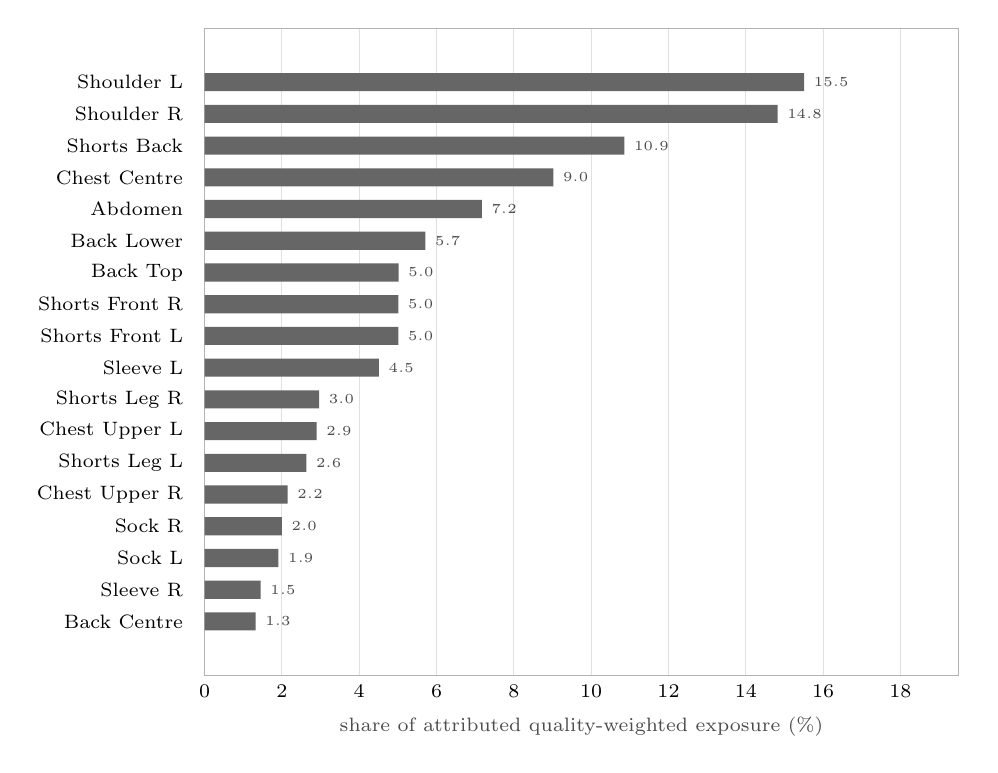
\begin{tikzpicture}
\begin{axis}[
  xbar, width=0.92\linewidth, height=98mm,
  xmin=0, xmax=19.5,
  symbolic y coords={Back Centre,Sleeve R,Sock L,Sock R,Chest Upper R,Shorts Leg L,Chest Upper L,Shorts Leg R,Sleeve L,Shorts Front L,Shorts Front R,Back Top,Back Lower,Abdomen,Chest Centre,Shorts Back,Shoulder R,Shoulder L},
  ytick=data, y dir=normal,
  bar width=2.3mm,
  axis line style={black!30},
  xmajorgrids, grid style={black!12},
  xlabel={share of attributed quality-weighted exposure (\%)},
  xlabel style={font=\scriptsize, color=black!70},
  tick label style={font=\scriptsize},
  ytick style={draw=none}, xtick style={draw=none},
  nodes near coords, nodes near coords align={horizontal},
  every node near coord/.append style={font=\tiny, color=black!70,
    /pgf/number format/fixed, /pgf/number format/fixed zerofill,
    /pgf/number format/precision=1},
]
\addplot[xbar, fill=black!60, draw=none] coordinates {
  (1.32,{Back Centre})
  (1.45,{Sleeve R})
  (1.91,{Sock L})
  (2.00,{Sock R})
  (2.15,{Chest Upper R})
  (2.63,{Shorts Leg L})
  (2.90,{Chest Upper L})
  (2.96,{Shorts Leg R})
  (4.51,{Sleeve L})
  (5.01,{Shorts Front L})
  (5.01,{Shorts Front R})
  (5.02,{Back Top})
  (5.71,{Back Lower})
  (7.17,{Abdomen})
  (9.02,{Chest Centre})
  (10.86,{Shorts Back})
  (14.82,{Shoulder R})
  (15.51,{Shoulder L})
};
\end{axis}
\end{tikzpicture}

\caption{\textbf{Where kit exposure actually accrues: share of quality-weighted
exposure per kit slot}, aggregated over eight full-highlight analyses
(\S\ref{sec:exp-counterfactual}; the ninth match is excluded after the attribution
audit described there, since its kept detections are not trustworthy). Percentages
are weighted by each match's attributed exposure and cover only detections the pose
stage could assign to a slot. The
distribution is strongly non-uniform — the two shoulder slots alone carry
$\sim$30\% of attributed exposure, an order of magnitude more than a sock slot —
which is exactly the structure a single flat placement multiplier cannot express.}
\label{fig:kitslots}
\end{figure}

\subsection{Exposure and EMV validation}
Fig.~\ref{fig:timeline} shows the per-sponsor exposure segments the pipeline recovers
for one full highlight video, which is the intermediate representation all exposure
and EMV figures are computed from. Beyond confirming end-to-end operation, the sorted
totals expose a commercially meaningful fact: on the same kit in the same match,
delivered exposure spans a 27$\times$ range (110\,s for the top sponsor to 4\,s for
the bottom one), driven largely by which slot each sponsor occupies
(Fig.~\ref{fig:kitslots}) — evidence that selling kit space at a flat rate
misprices most of it. To validate the measurement itself,
we compare system-computed exposure-seconds against an independent manual timing of
logo appearances for at least one full match. We report EMV as a downstream consequence
of this validated exposure measurement rather than as independently verified: CPM,
audience size, and placement multiplier are deployment-supplied business inputs, not
measurable ground truth, so multiplying by them is arithmetic rather than something to
validate against an external reference — unless an independent buyer valuation is
available for direct comparison, which would be a stronger, separate claim.
\TODOnum{Report exposure-seconds MAE against manual ground truth.}

\subsection{Placement-level exposure in deployment}
Fig.~\ref{fig:kitslots} reports the measured per-slot exposure distribution that
placement-level pricing (C3) is built on. Two observations matter for pricing. First,
the distribution is far from uniform: shoulder and chest-adjacent slots dominate
attributed exposure, while sleeve, sock, and back-centre slots individually carry
under 2\% each — supporting the practice of pricing slots differently, but from
measurement rather than convention. Second, the ordering is not the conventional
price ordering: in this deployment the shorts-back slot outranks chest-centre,
an artefact of how the club's own pitch-side camera views play, and precisely the
kind of deployment-specific evidence a flat industry multiplier cannot anticipate.

\subsection{Accessibility evidence}
\TODOnum{Report end-to-end processing time (video-minutes processed per wall-clock
minute) on one named, commodity hardware configuration, and the approximate annotation
time spent per sponsor class using the model-assisted labelling loop of
\S\ref{sec:method}.} These two numbers are the primary quantitative support for the
accessibility claim in this paper and are prioritized for measurement before submission.

% ============================================================================
\section{Discussion and Limitations}
\label{sec:discussion}

Team attribution assumes a stable kit within a match; a mid-season kit change requires a
reference refresh. Colour-and-embedding fusion for team classification has not yet been
stress-tested across a wide range of lighting conditions, and this is not hypothetical:
in one night fixture in our deployment, the classifier systematically assigned the
target club's own white kit to the opponent class even though the stored reference
features were correct (\S\ref{sec:exp-counterfactual}) — silently deleting most of that
match's genuine sponsor exposure. Because the failure direction is revenue-critical, a
deployment should monitor the per-match exclusion rate and treat an outlier (here,
78\% against a fleet median near 40\%) as a signal for human review rather than as a
valid measurement. Because the framework targets
self-captured video rather than official broadcast feeds, it must also tolerate a wider
range of camera stability, framing, and production quality than prior systems evaluated
only on broadcast-sourced footage; we have not yet characterized detection or
team-attribution robustness across this range of capture sources (e.g.\ a fixed
pitch-side camera vs.\ a hand-held recording), and flag this as an open question rather
than a validated property. The sparse sampling rate used
for the analytics pass trades exposure-time precision for processing cost; we report the
resulting worst-case timing error explicitly rather than treat sampling as free.
Manual annotation, while reduced by the model-assisted loop, remains a real,
non-eliminated cost when onboarding a new sponsor class, and is the main residual
barrier to the accessibility claim in this paper (\S\ref{sec:future}). As discussed in
\S\ref{sec:related-pricing}, our placement-level pricing addresses one specific,
well-documented weakness of AVE-style valuation (arbitrary multipliers) but not the
broader critique that such metrics do not capture audience quality, sentiment, or
brand-recall impact; we do not claim to have solved sponsorship valuation, only to have
made one component of it less arbitrary and more transparent.

\textbf{Data and ethics statement.} The framework is designed around video that a club
captures and uploads itself, which removes the third-party broadcaster copyright
concerns that would apply to processing official broadcast feeds; the club retains
ownership of its own footage. The system nonetheless processes images of real players,
so consent/data-handling practice still matters. \TODOnum{state precisely what
permission or policy governs use of a club's own match footage for this research, and
for any figures published in the paper.} Players are tracked only as anonymous
instances for the purpose of kit-slot attribution, not for personal identification; the
system's output is brand and media-value analytics, not player-performance or
biometric data.

% ============================================================================
\section{Future Work}
\label{sec:future}

The main remaining barrier to full accessibility is the manual annotation effort
required per sponsor class. We are separately exploring an annotation-free direction
that exploits a structural property of team sports: a club wears one fixed kit for an
entire season, and advertising boards are physically static, so each distinct
logo-bearing surface could, in principle, be identified once — at its clearest
occurrence in the available footage — and propagated to every other occurrence by
tracking and geometry rather than by repeated visual classification. Early internal
results on this direction are encouraging but preliminary, and are explicitly not part
of the claims made in this paper. Other directions include synthetic data generation for
rare viewing conditions, and a more detailed, audience-quality-aware model for
converting measured exposure into media value, directly addressing the deeper AVE
critique noted in \S\ref{sec:discussion}.

% ============================================================================
\section{Conclusion}
\label{sec:conclusion}

We present an open, self-hosted framework for sponsor exposure and media-value
measurement that addresses two problems left open by prior published work — attribution
of logos shared between competing teams, and pricing at the level of individual kit
placements — while remaining deployable without an enterprise vendor contract or an
in-house machine-learning team. We position our pricing methodology explicitly against
both the manual AVE/EMV tradition and recent AI-driven valuation systems, and are
transparent about which part of the well-documented criticism of media-value-equivalency
metrics our contribution does, and does not, address. The framework is deployed and
evaluated on a real professional club, which grounds the accessibility claim in an
actual deployment rather than in argument alone.

% ============================================================================
\bibliographystyle{IEEEtran}
\bibliography{refs_accessibility}

\end{document}
